\documentclass{article}

\usepackage{amssymb,amsmath,multicol,enumerate,amsthm,graphicx}

\usepackage{enumerate}
\usepackage{color}
\usepackage{xcolor}
\usepackage{listings}
\usepackage{mathtools}
\usepackage{graphicx}
\graphicspath{ {./} }
\usepackage{pgfplots}
% \usepackage{./bluespec}
\usepackage{svg}
\usepackage[ddMMyyyy]{datetime}
\usepackage{graphicx} % Required for inserting images
\usepackage[margin=1in]{geometry}   % Marges
\usepackage{latexsym}
\usepackage{amssymb}
\usepackage{amsmath}
\usepackage{amsfonts}
\usepackage{verbatim}
% \usepackage{listings}
\DeclareSymbolFont{largesymbols}{OMX}{cmex}{m}{n} % However for large sigmas we want the Computer Modern symbol
\renewcommand{\ttdefault}{cmtt}
\usepackage{array}
\usepackage{multirow}
\usepackage{color}
\usepackage{xspace} % xspace takes care of the \@ after a capitalized word before a period.
\usepackage{multicol}
\usepackage{graphicx}
\usepackage{fancyhdr}
\usepackage{hyperref}

\setlength{\oddsidemargin}{0pt}
\setlength{\evensidemargin}{0pt}
\setlength{\textwidth}{6.5in}
% \setlength{\topmargin}{-1in}
% \setlength{\bottommargin}{-1in}
% \setlength{\textheight}{8.5in}
% \usepackage[margin=1in]{geometry}
\setlength{\parskip}{1pc}
\setlength{\parindent}{0pt}

\lstdefinelanguage{RSVAssembler}
{
  alsoletter={.}, % allow dots in keywords
  alsodigit={0x}, % hex numbers are numbers too!
  morekeywords=[1]{ % instructions
    lb, lh, lw, lbu, lhu,
    sb, sh, sw,
    sll, slli, srl, srli, sra, srai,
    add, addi, sub, lui, auipc,
    xor, xori, or, ori, and, andi,
    slt, slti, sltu, sltiu,
    beq, bne, blt, bge, bltu, bgeu,
    j, jr, jal, jalr, ret,
    scall, break, nop
  },
  morekeywords=[2]{ % sections of our code and other directives
    .align, .ascii, .asciiz, .byte, .data, .double, .extern,
    .float, .globl, .half, .kdata, .ktext, .set, .space, .text, .word
  },
  morekeywords=[3]{ % registers
    zero, ra, sp, gp, tp, s0, fp,
    t0, t1, t2, t3, t4, t5, t6,
    s1, s2, s3, s4, s5, s6, s7, s8, s9, s10, s11,
    a0, a1, a2, a3, a4, a5, a6, a7,
    ft0, ft1, ft2, ft3, ft4, ft5, ft6, ft7,
    fs0, fs1, fs2, fs3, fs4, fs5, fs6, fs7, fs8, fs9, fs10, fs11,
    fa0, fa1, fa2, fa3, fa4, fa5, fa6, fa7
  },
  morecomment=[l]{;},   % mark ; as line comment start
  morecomment=[l]{\#},  % as well as # (even though it is unconventional)
  morestring=[b]",      % mark " as string start/end
  morestring=[b]'       % also mark ' as string start/end
}


\lstset{language=Verilog,keywordstyle={\bfseries \color{blue}}}

\definecolor{mygreen}{rgb}{0,0.6,0}
\definecolor{mygray}{rgb}{0.5,0.5,0.5}
\definecolor{mymauve}{rgb}{0.58,0,0.82}
\definecolor{codegreen}{rgb}{0,0.6,0}
\definecolor{codegray}{rgb}{0.5,0.5,0.5}
\definecolor{codepurple}{rgb}{0.58,0,0.82} 
\definecolor{backcolour}{rgb}{0.95,0.95,0.92}


\lstset{ %
  backgroundcolor=\color{white},   % choose the background color
  basicstyle=\footnotesize,        % size of fonts used for the code
  breaklines=true,                 % automatic line breaking only at whitespace
  captionpos=b,                    % sets the caption-position to bottom
  commentstyle=\color{mygreen},    % comment style
  escapeinside={\%*}{*)},          % if you want to add LaTeX within your code
  % morekeywords=[1]{arg,pos},
  keywordstyle=\color{blue},       % keyword style
  stringstyle=\color{mymauve},     % string literal style
  backgroundcolor=\color{backcolour},   
    commentstyle=\color{codegreen},
    keywordstyle=\color{magenta},
    numberstyle=\tiny\color{codegray},
    stringstyle=\color{codepurple},
    basicstyle=\ttfamily\footnotesize,
    breakatwhitespace=false,         
    breaklines=true,                 
    captionpos=b,                    
    keepspaces=true,                 
    numbers=left,                     
    numbersep=5pt,                  
    showspaces=false,                
    showstringspaces=false,
    % keywordstyle=\color{weborange},
    showtabs=false,                  
    tabsize=2
}




\title{6.111 Block Diagram Report: \\ FPGA-based Accelerator for Vector Search}
\author{Lasya Balachandran, Sanjay Seshan\\lasyab@mit.edu, seshan@mit.edu}
\date{\today}

\begin{document}

\maketitle


    % A high level (no need to dig too deep yet) specification of what your project should do. This can absolutely be tweaked and tuned over the course of the next couple of days.
    % A discussion what the system's use cases are, how it should behave, and what its desired properties are (i.e., how does this system benefit from being run on an FPGA?)
    % Design goals for your project - what properties are you prioritizing for? What components do you need to build in order to bring together a minimal viable product?
    % How work will be broken up to ensure everyone can always be working efficiently.

\section{Abstract}
With the application of graphs in large-scale modeling, such as social network analysis and image and video segmentation, among other applications, graphs are increasingly being used to encode and find complex relationships between data for machine learning models, leading to an increased need for optimization of these models. As a result, in order to better support model-specific algorithm efficiency, there has been work to create specialized hardware accelerators focusing on aspects such as memory accessing, latency, and resource allocation. However, current accelerators for graph problems are not scalable and can only be optimized for a single algorithm, such as graph random walks or matrix multiplication. 

The goal of this project is to implement an accelerator for a general-use search algorithm. One of the main problems when working with large graphs is the large amount of computations, which is a reason why current accelerators have focused on optimizing only a single algorithm. One way we can reduce these computations is by running the calculations on only a subset of the graph. For example, the novel graph-based vector search algorithm iQAN uses a priority queue of certain length to approximate the most similar points and avoid brute-force-checking all of the points [1]. Graph sampling, where we select a random subset of vertices representative of the entire graph, can also be used to reduce a graph.

% One way to reduce computation is by graph sampling, where we select a random subset of vertices representative of the entire graph, when traversing the graph from a starting set of nodes, but sampling graphs, or reducing them, is hard to perform efficiently. 

Due to the reprogrammability of FPGAs and following from previous work on hardware and software co-design for an inverted file index (IVF)-product quantization (PQ)-based vector search algorithm on FPGAs, we propose an FPGA-based accelerator that builds off of the iQAN and graph sampling framework to provide an interface to efficiency search graphs [2]. 
% This system will work to provide a general interface for graph sampling and pattern search problems. 
Some applications of this system include graph-based vector search (e.g. iQAN) for machine learning applications and graph pattern mining on the sampled graphs.

This project will build on the work of iQAN (graph-based vector search) and NextDoor (efficient graph sampling on GPUs) [1, 3]. It is also part of our UROP with Arvind and Xuhao Chen in the Computation Structures Group at CSAIL.


% \newpage
\section{Algorithm}
Based on the paper on iQAN, we will be implementing the Best-First Search (BFiS), a graph-based vector search algorithm, on the FPGA. The algorithm is as follows:

\begin{lstlisting}[language=c]
Input: graph G, starting point P, query Q, queue capacity L
Output: K nearest neighbors of Q
priority queue S <- {} /* sorted based on distance */
index i <- 0
compute dist(P, Q)
add P into S
while S has unchecked vertices do /* stop condition */
    i <- the index of the 1st unchecked vertex in S
    mark v_i as checked
    foreach neighbor u of v_i in G do
        if u is not visited then
            mark u as visited
            compute dist(u,Q)
            add u into S /* u is unchecked */
    if S.size() > L then S.resize(L)
return the first K vertices in S
\end{lstlisting}


Source: iQAN paper \href{https://johnpzh.github.io/assets/papers/PPoPP-2023_iQAN_Zhen.CameraReady.pdf}{https://johnpzh.github.io/assets/papers/PPoPP-2023\_iQAN\_Zhen.CameraReady.pdf}.
      
\section{Block Diagram}

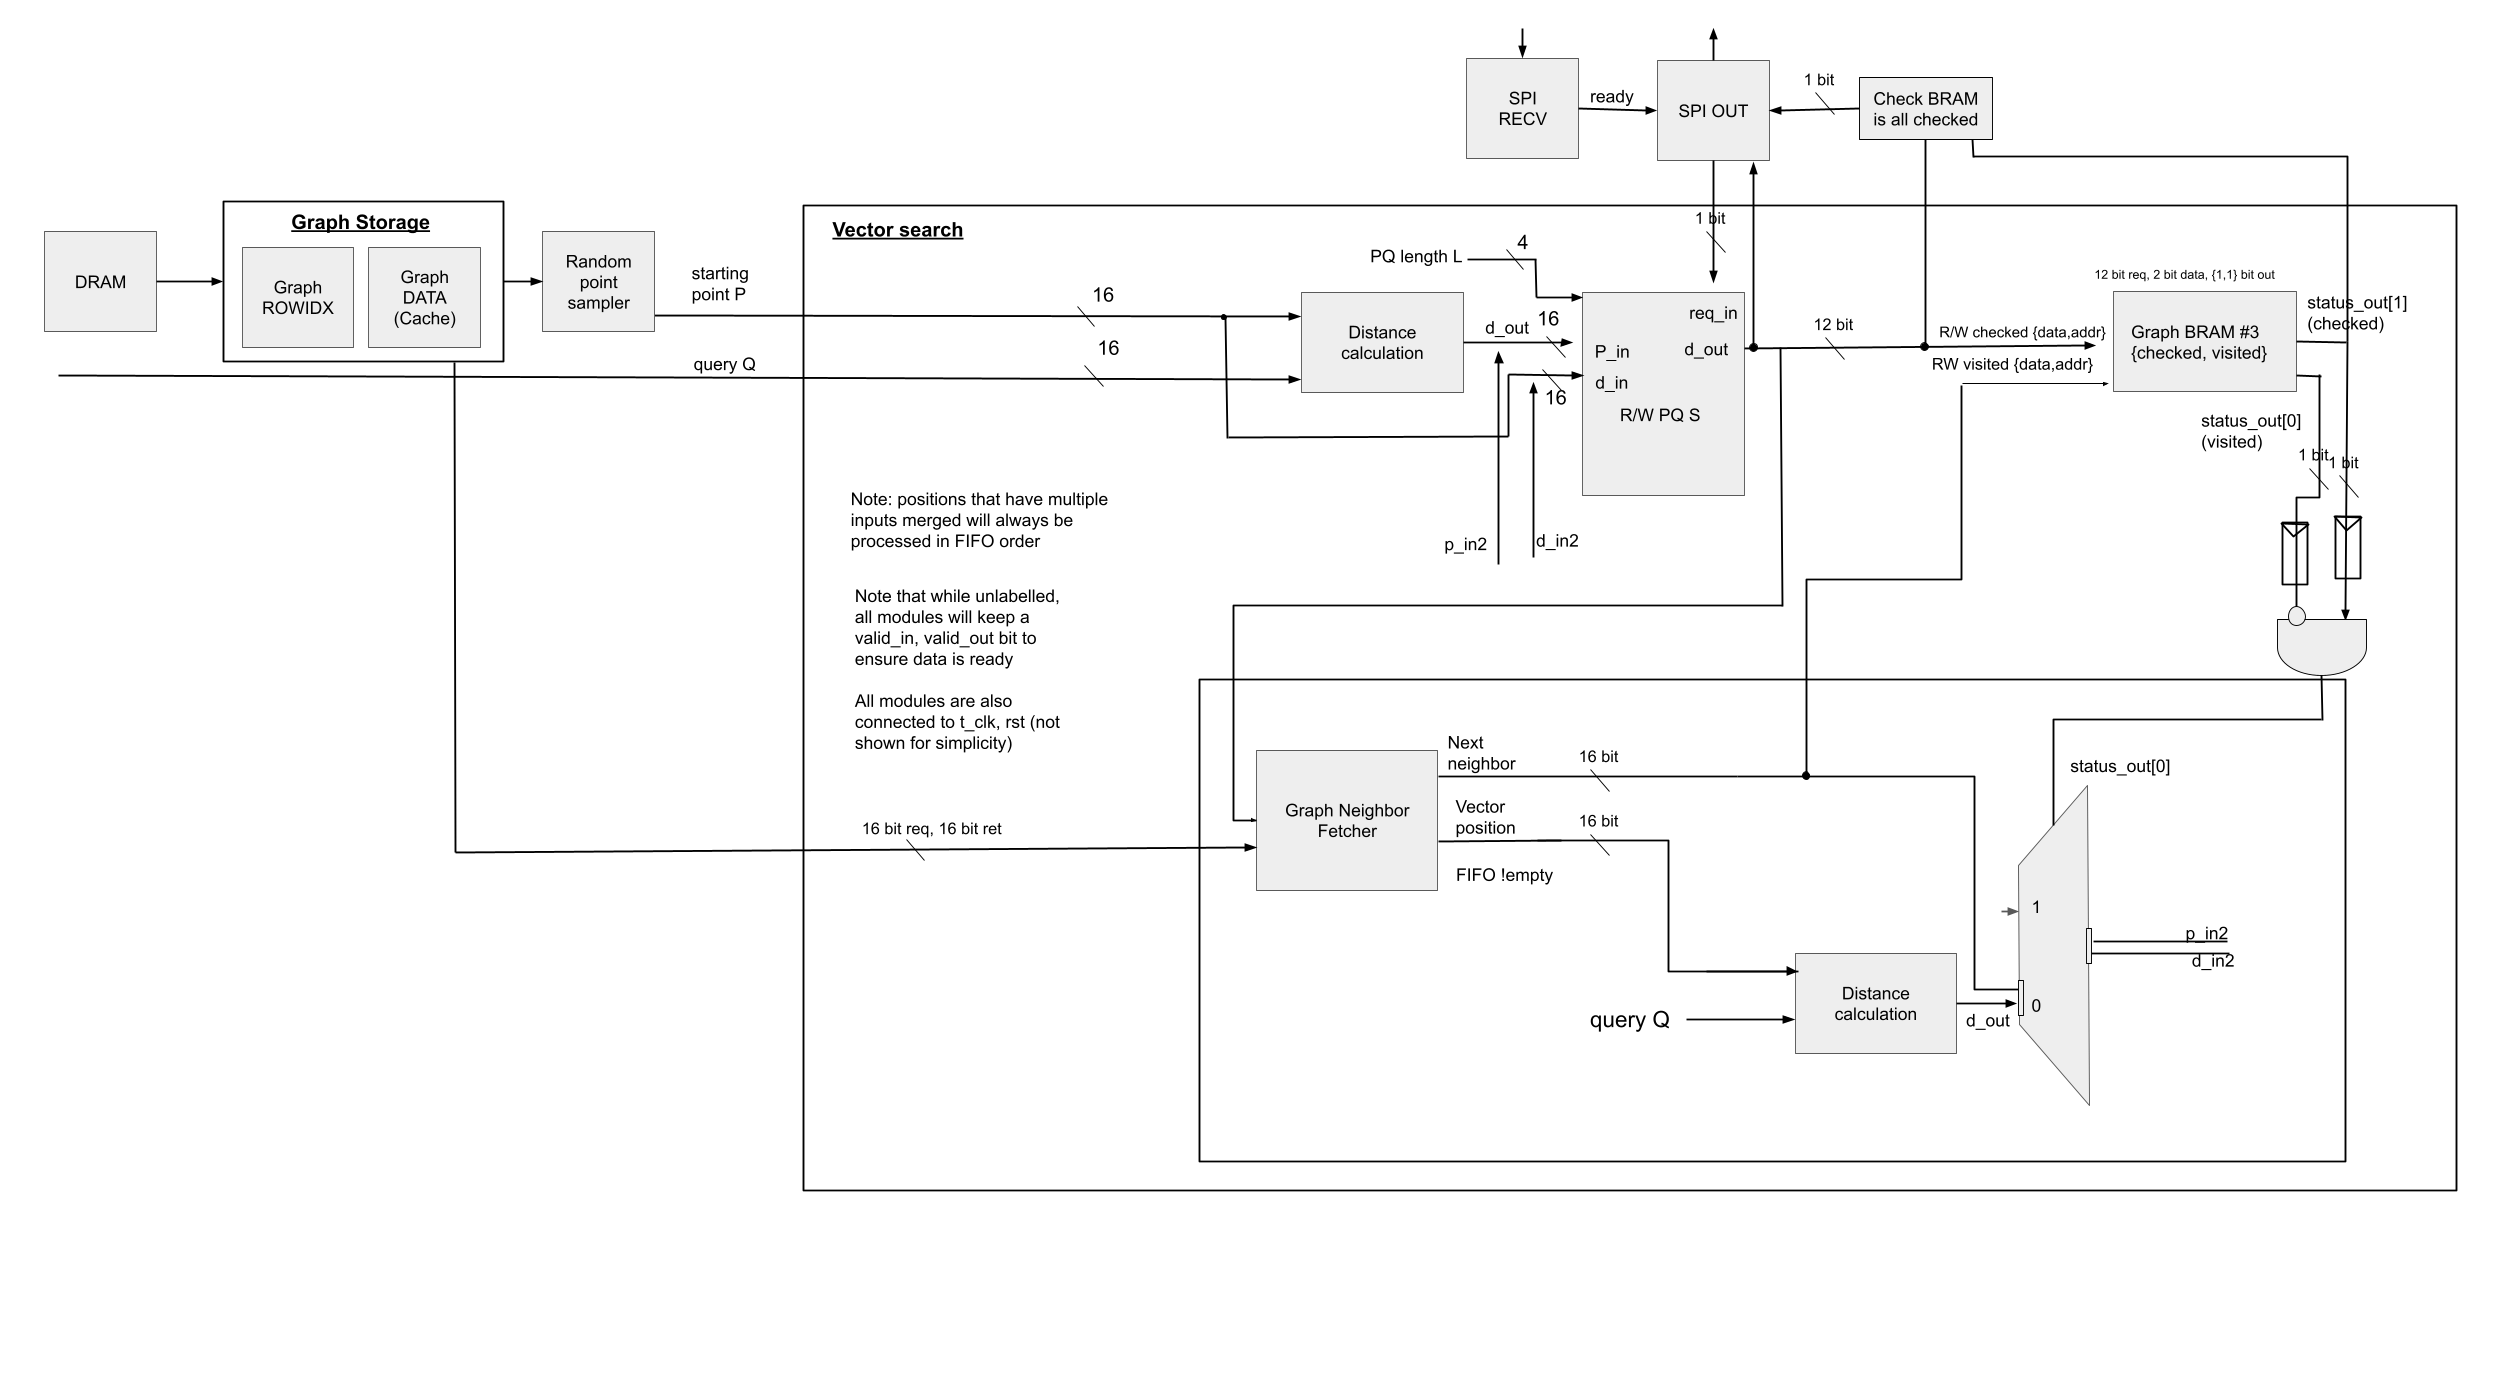
\includegraphics[width=18cm]{BlockDiagram2.png}

Our design is composed of three main components: graph storage, vector search, and SPI output. The vector search module is a much larger module that is composed of several different modules.


\section{Storing Graph and Preprocessing}

We plan to store our graphs using BRAM in the Compressed Sparse Row (CSR) format. A traditional approach to storing graphs is to use an Adjacency Matrix that has dimensions $n\times n$ for $n$ vertices in the graph. Each row would contain a 1 or 0 at each column to determine if that entry is a neighbor of the desired vertex. This approach results in an upper triangular matrix, which consumes a lot of space. While an Adjacency Matrix would work well for dense graphs, most realistic graphs are sparse, so we opt to use Compressed Sparse Row (CSR) instead.

A CSR formatted graph contains a row pointer, a list of neighbor ids, and node values. The row pointers point to sequential positions in the neighbor (colidx) array. This representation is far more efficient than an adjacency matrix. The following diagram is a good example of the CSR format, derived from an adjacency matrix.

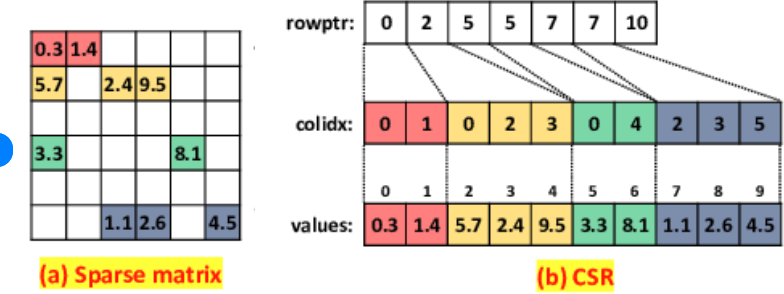
\includegraphics[width=10cm]{csr_eg.png}

Source: \href{https://www.researchgate.net/figure/CSR-and-DCSR-formats_fig2_325706323}{https://www.researchgate.net/figure/CSR-and-DCSR-formats\_fig2\_325706323}

We will pre-process these graphs in software to form the CSR format. 

\subsection{BRAMs and Compressed Sparse Row (CSR) Format}

We plan to store our graphs on the FPGA using 2 BRAM modules. 

The first will store the row pointers, where each index in the rowptr corresponds to its position/address in the other bram. Each entry will be 16 bits wide, with number of rows being the size of the graph $g.size()$, or an address space of $\log_2(g.size())$ bits.

We will use a slight augmentation on the traditional CSR software design as shown above. To be specific, we are looking to merge the data array and neighbor array and allow reverse lookup from address to vertex ID. Below is the condensed representation that we will use to identify components of a graph:

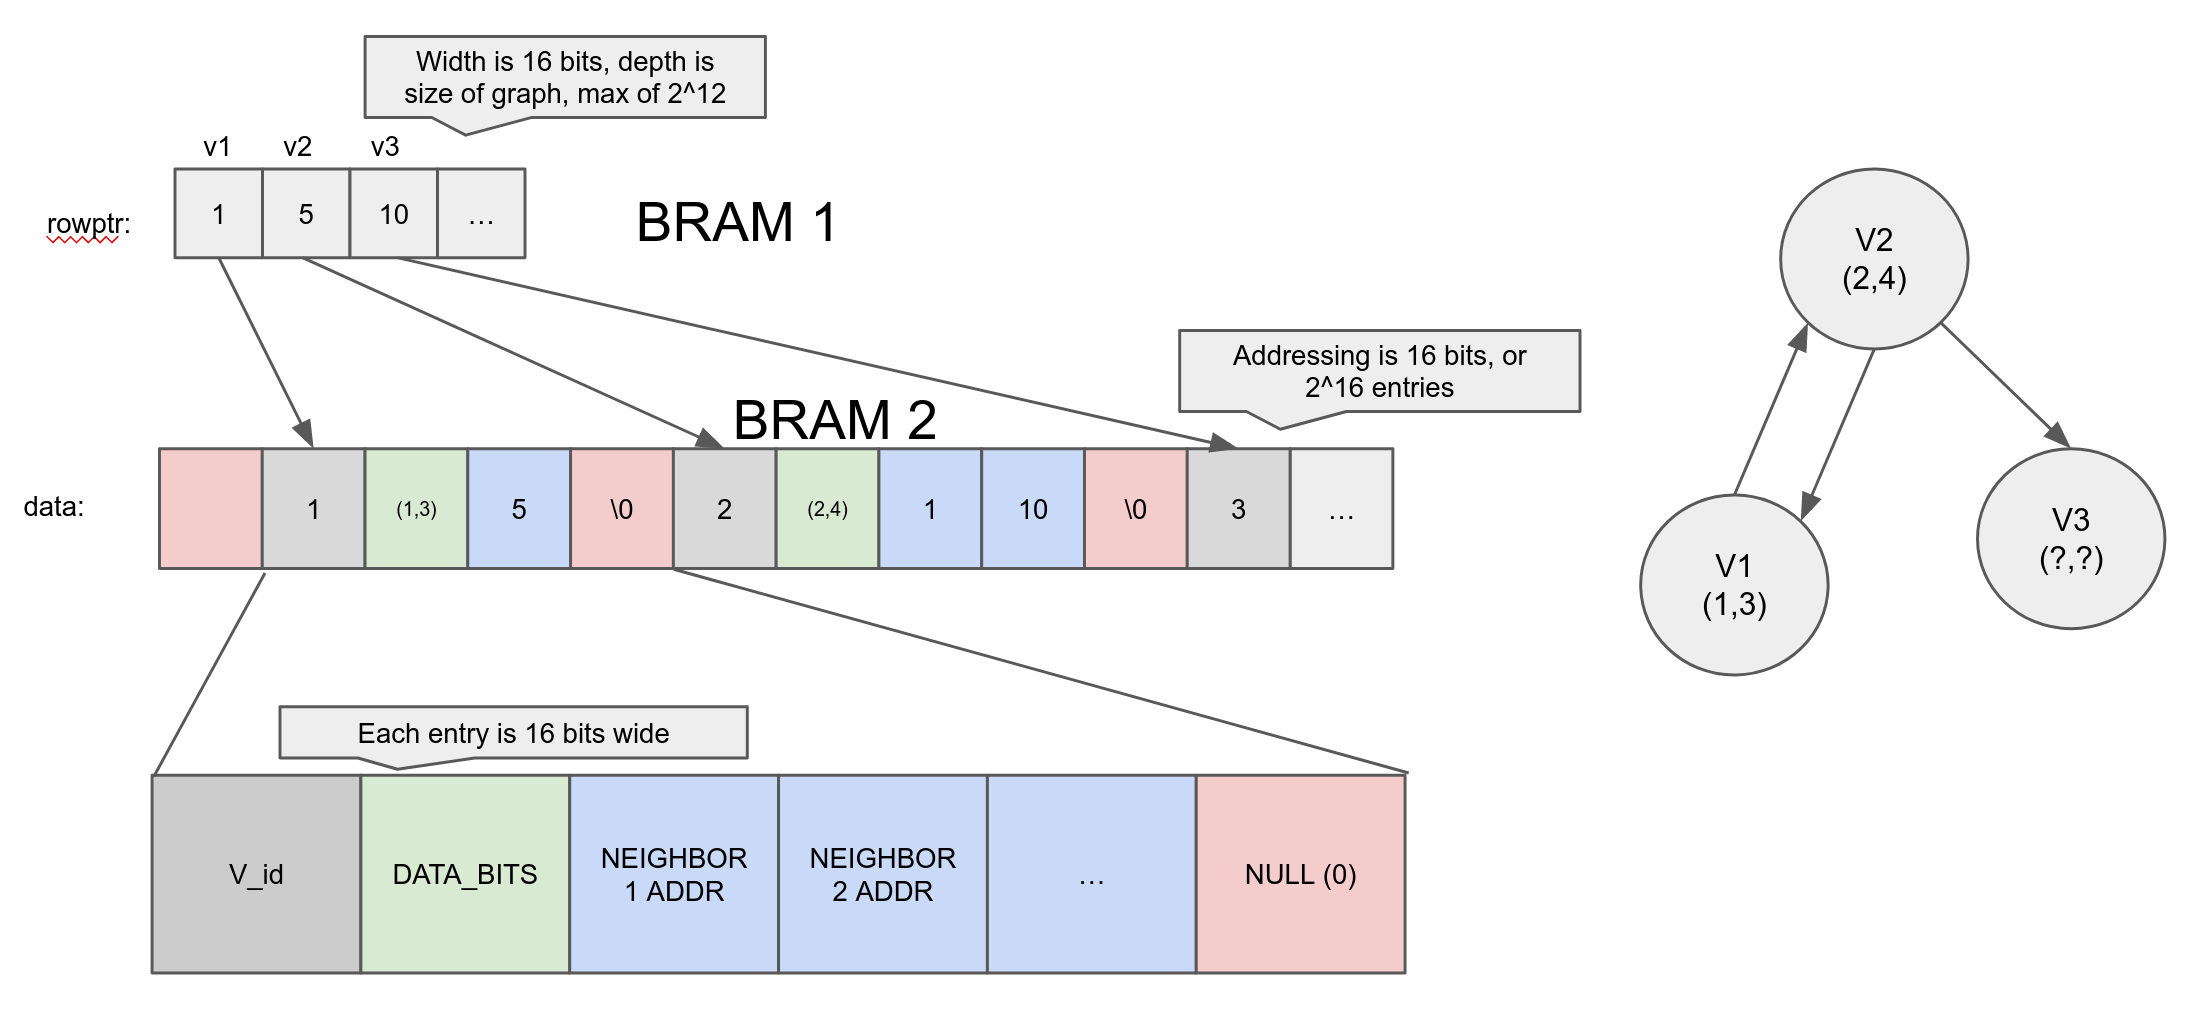
\includegraphics[width=12cm]{csr_entry.png}

The corresponding graph is shown at right. The number of neighbors is dynamic, and can be grown, memory space permitting. This CSR format contains all necessary information to conduct a vector search. Note that neither v0 nor the 0 data address exist, since we use 0 as our NULL termination.

Our two BRAMs will be 16 bit width, with one having $2^{12}$ valid entries and the other having $2^{16}$ valid entries. It is important to note that graph inputs are read only. 

We also plan to store the status of checked and visited vertices in the vector search in a third BRAM. It will have the same depth as BRAM 1 ($2^{12}$ bits), but a width of 2 (\{checked, visited\}) bits instead of 16. The format will otherwise remain identical to BRAM 1 (rowidx). This part is to simply avoiding writing to the same BRAM that stores the graph cache.

\subsection{Updating Graph}

The BRAMs will be populated with the graph upon flashing. If this is not possible, we will use the SPI communication tool from lab to transfer graph information and write it to the BRAMs at reset, using an external programmable microcontroller.

We understand that most graphs will be larger than the available BRAM size. Our long term goal is to get DRAM working to store larger graphs, with the data BRAM 2 module functioning as cache for the larger dataset. Vertex IDs should still fit inside the BRAM. 

An example cache we would implement is as follows (source: \href{https://www.sciencedirect.com/topics/computer-science/set-associative-cache}{https://www.sciencedirect.com/topics/computer-science/set-associative-cache}:

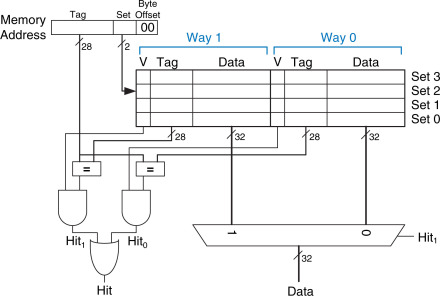
\includegraphics[width=6cm]{cache.jpg}

However, to start, we will use the lab2 SPI protocol to request an address and return the appropriate line of data. This would be a drop in replacement for DRAM until we finish the DRAM protocol. In this case, we will allow more than 16 bits for the vector position, such as 32*10 bits, for 10 component float positions.

For the minimum viable product, we will assume we can fit a graph in BRAM. 

\subsection{Random Sampling for Starting Point}

This section is not needed for the minimal viable product and will only be added time permitting. At the moment, we see this module selecting a small random subset of vertices (possibly using an LFSR) from BRAM 1, computing the distances between each vertex and the query, and using the one with the smallest distance as the starting point. Choosing a starting point in this way would likely allow the algorithm to finish running in less iterations.

For the minimal viable product, the starting point can be calculated before-hand, using a software sampler.

\section{Graph-based Vector Search}
Our vector search module will likely be the largest component of this project and will consist of several different modules. We plan on using a state machine with 7 states (subject to change) for this module and will use three separate modules (calculate distance, update priority queue $S$, and find neighbors of a given point). 

\subsection{Finite State Machine}
In the diagram below, our $P$ represents our starting point, $Q$ represents the query, $S$ represents the priority queue, and $k$ represents the number of points we want to return.

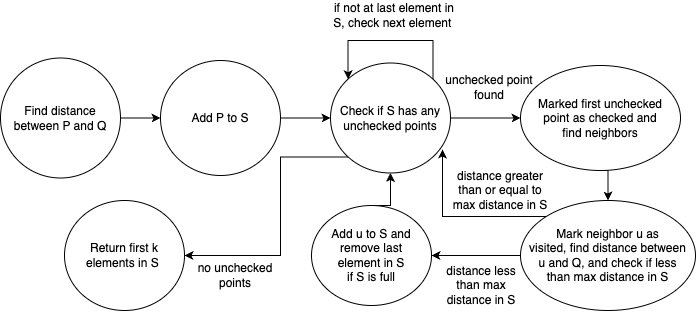
\includegraphics[width=16cm]{FSM.drawio.png}

This state machine is largely based on the pseudocode in section 2. We initially find the distance between $P$ and $Q$ and add the point to $S$. The next 4 states represent the while loop, where we first check if $S$ has any unchecked points. If we do not find any unchecked points, we will return the first $k$ elements in $S$, which will correspond to the $k$ elements with the highest priority. If we find an unchecked point (checked register is 0), we will run the inner loop on the neighbors of the point.

\subsection{Calculating Distance Between Point and Query}

Our fetcher module returns the n-dimension position vector $\vec v$. We are given the query position as an input, so we already have its position vector as a constant. We will then use the Euclidean distance algorithm to get the desired value. We will initially set the size of the vectors at compile time (e.g. 4 dimensions of 4 bits each). We may decide later to handle sizes dynamically, which would be done in multiple cycles. We might also increase the number of bits allocated for data for larger graphs. 

$$\text{dist}(\vec v) = ||\vec v||$$
$$=\text{dist}(x_1,y_1,x_2,y_2+\dots)=\sqrt{(x_1-x_2)^2+(y_1-y_2)^2+\dots}$$

However, to avoid implementing square root, we can just consider the square distance anywhere dist is used.

$$\text{dist}^2(x_1,y_1,x_2,y_2,\dots)=(x_1-x_2)^2+(y_1-y_2)^2+\dots$$

Based on timing constraints, we may need to implement a multicycle, pipelined multiplier to handle the squares, but we will just use the default SystemVerilog multiply implementation for now.

\subsection{Updating Priority Queue}
The priority queue will have a fixed size and will store the closest $L$ elements visited. 

There are a few Priority Queue architectures that we can consider: BRAM-based, searchable FIFO-based, or dynamically grown array (BRAM) based.  
% : FIFO-based, Shift Register, Systolic array.

% We opt to use a Systolic array based priority queue.  

Since we initially expect to have a limited size ($<$10 elements), we will opt to use a simple searchable FIFO based priority queue. This is basically an array search at each read.

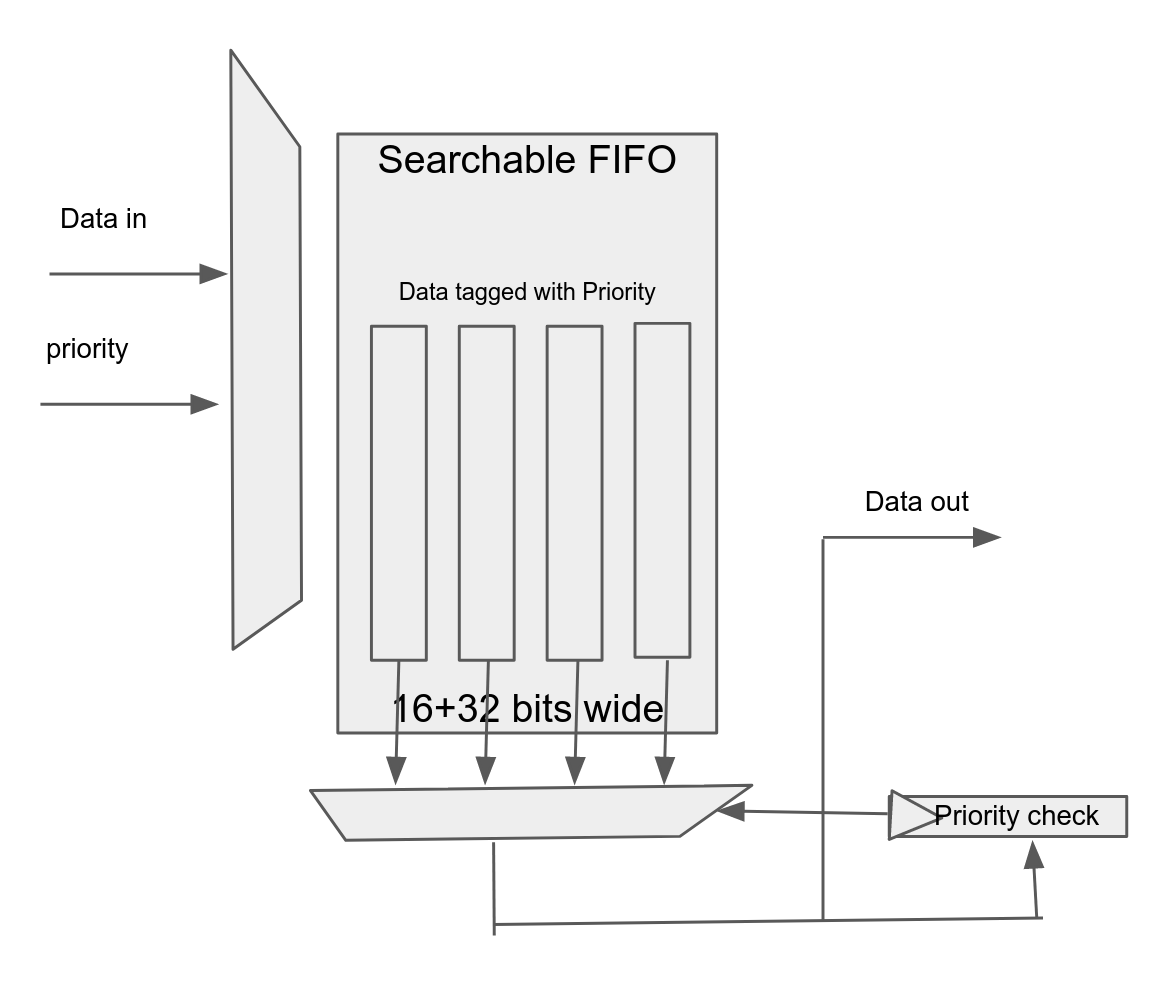
\includegraphics[width=8cm]{pq2.png}

In order to add an element to the priority queue, we will insert a tagged entry with \{data address in, priority\}, totaling at 16+32 bits. To read, each element will be checked in the queue to be the highest priority before dequeuing it. That freed position is now available for insertion. This process will repeat to enqueue and dequeue into the priority queue.

% 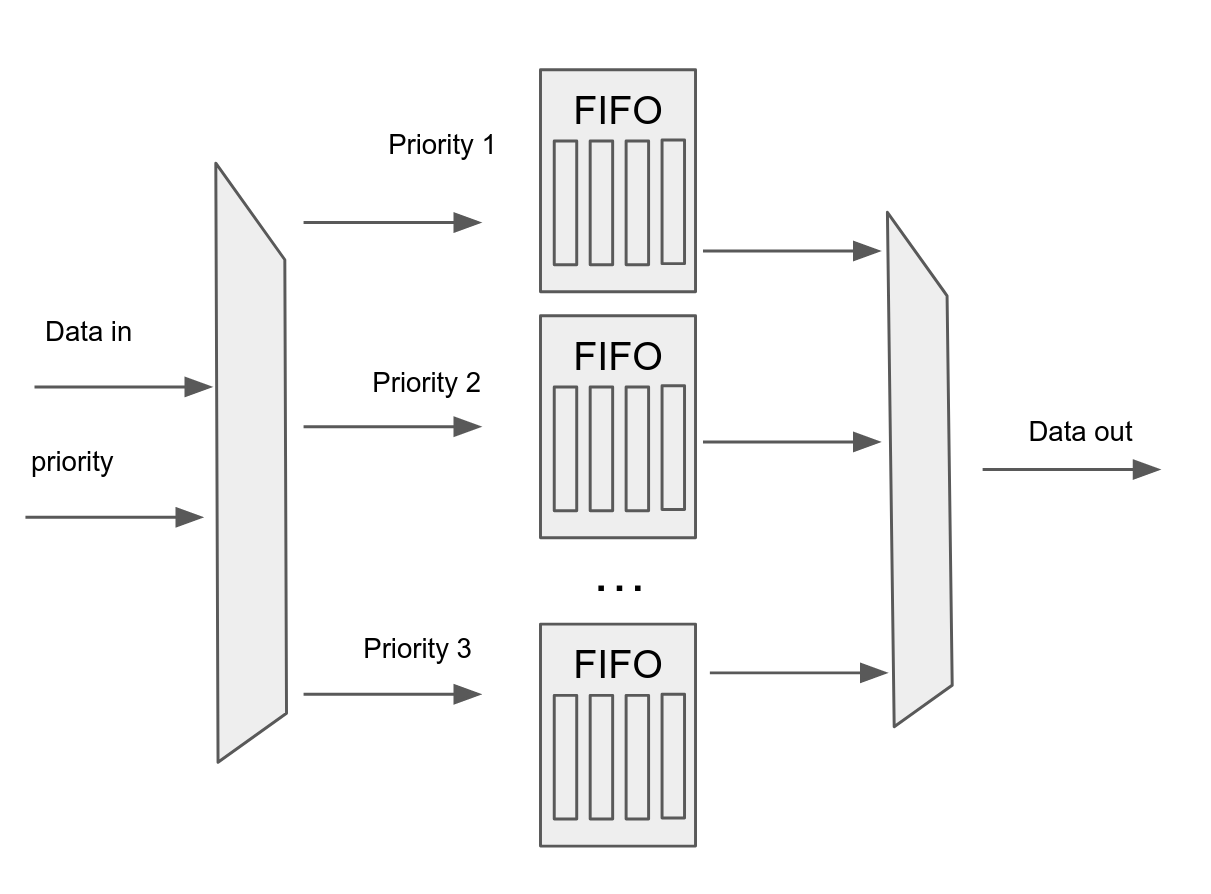
\includegraphics[width=6cm]{pq.png}

After the minimal viable product is produced, we will implement the priority queue in BRAM, for dynamically allocated size. This will be a fixed size BRAM, though sufficiently large, with elements ordered like a binary search tree, for quick access.

% We may need to consider some alternative, more efficient designs, such as those listed at\\ \href{https://ece.uwaterloo.ca/~arrmorto/pubs/fpl07Poster.pdf}{https://ece.uwaterloo.ca/$\sim$arrmorto/pubs/fpl07Poster.pdf}, if our design were to have a bottleneck at the priority queue.

\subsection{Finding Neighbors of Point}

For any given point, we can look up its address using the rowptr array, as defined in Section 4.1. For vertex ID $N$, we request a read from the rowptr BRAM at index N. We wait two cycles and use the returned address ADDR to send a read request into the data array. To get the position for distance calculation, we request ADDR+1. Then we will continue to get the N neighbors, which are stored in ADDR+2 to ADDR+2+N. N is increasing at each read iteration, and its maximum is determined from the number of elements between ADDR+2 and the termination NULL (0) pointer.

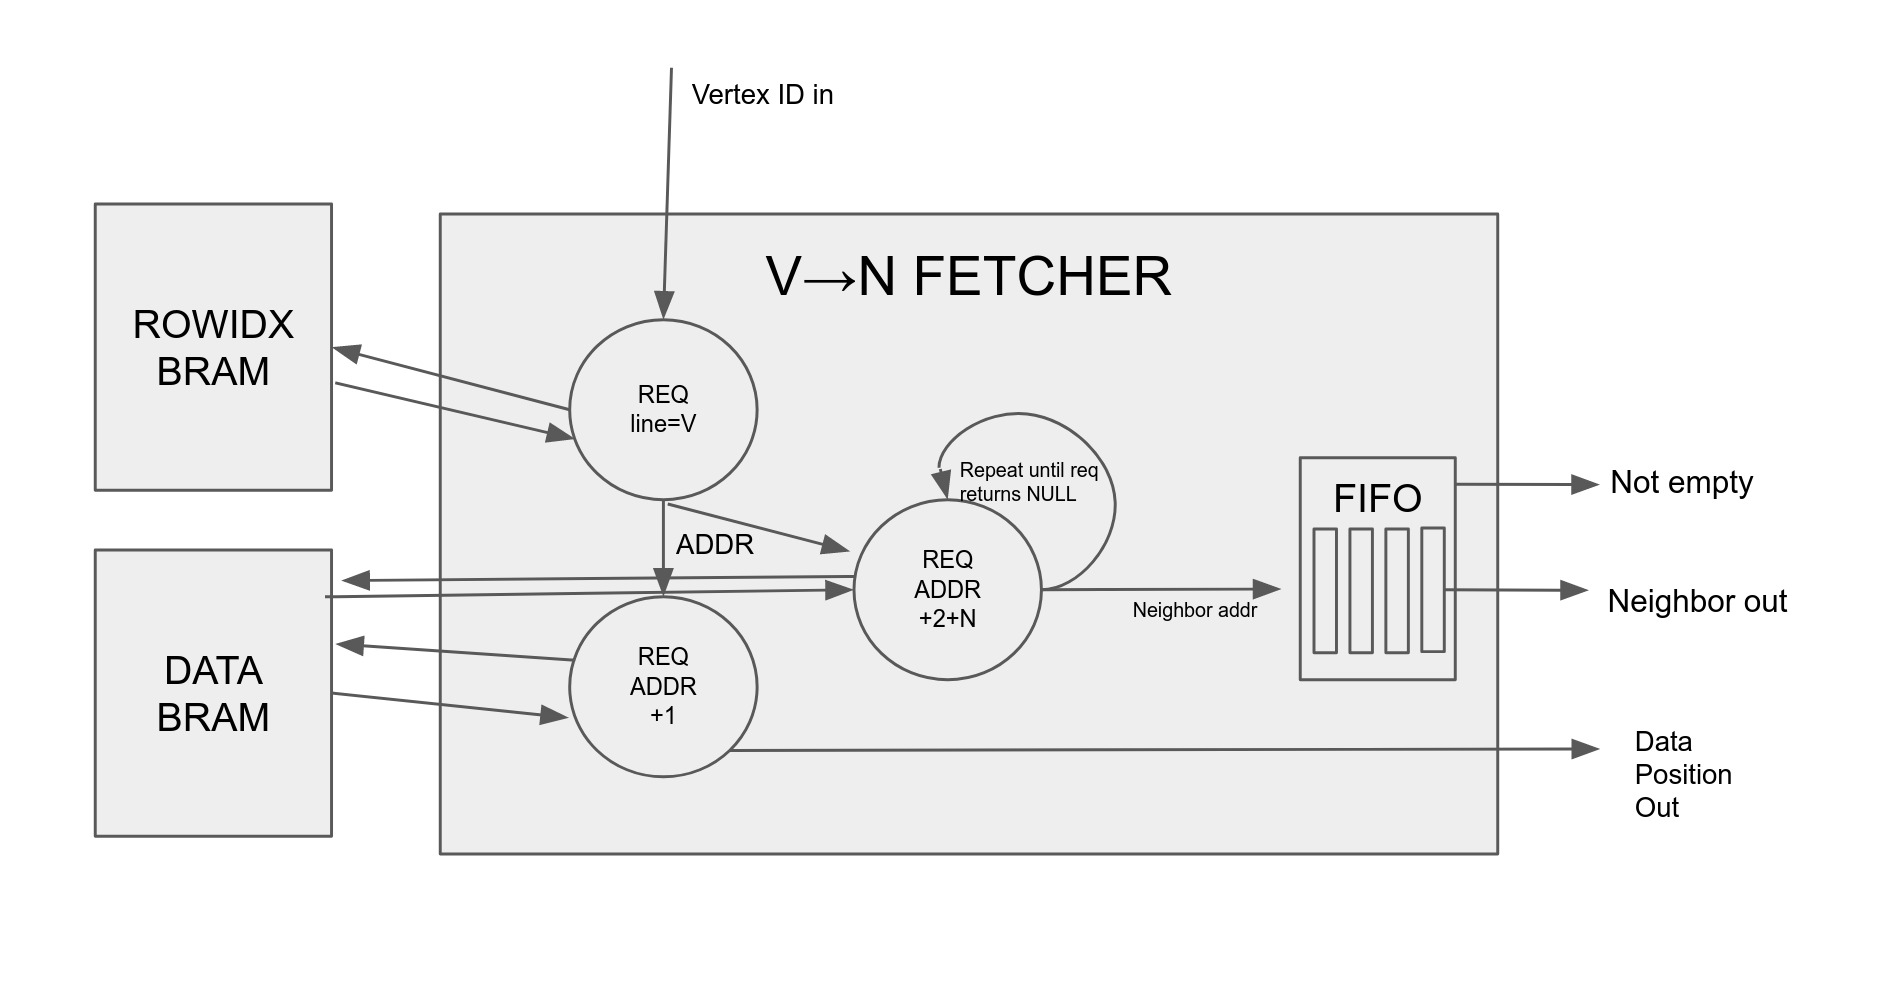
\includegraphics[width=15cm]{fetch.png}


The fetching of neighbors will run asynchronously. Specifically, after the first neighbor read request is initiated, we will continue fetching subsequent addresses, storing them in a FIFO queue, to be read by the user until empty (NULL termination). The FIFO queue will be fixed-size, and elements will be loaded only when space is available. We will keep the FIFO around the average number of neighbors. To start, we will experiment with size 4. When the FIFO is full, read requests will continue to be delayed until elements are popped. The FIFO does not need to be emptied before starting to read the next vertex data. Note that while it is not depicted in the diagram for simplicity, each read request will include a delay of 2 cycles for BRAM to return. FIFO reads, however, are single cycle. The neighbor can dequeue/pop when data is ready/FIFO is not empty.


\section{System Output}
% FILL IN -- dump memory out over SPI? copy spi diagram from lab?
The top $N$ elements from the priority queue will be dumped over SPI. The data line will be connected to the read port on the priority queue and transmitted to the receiving machine.

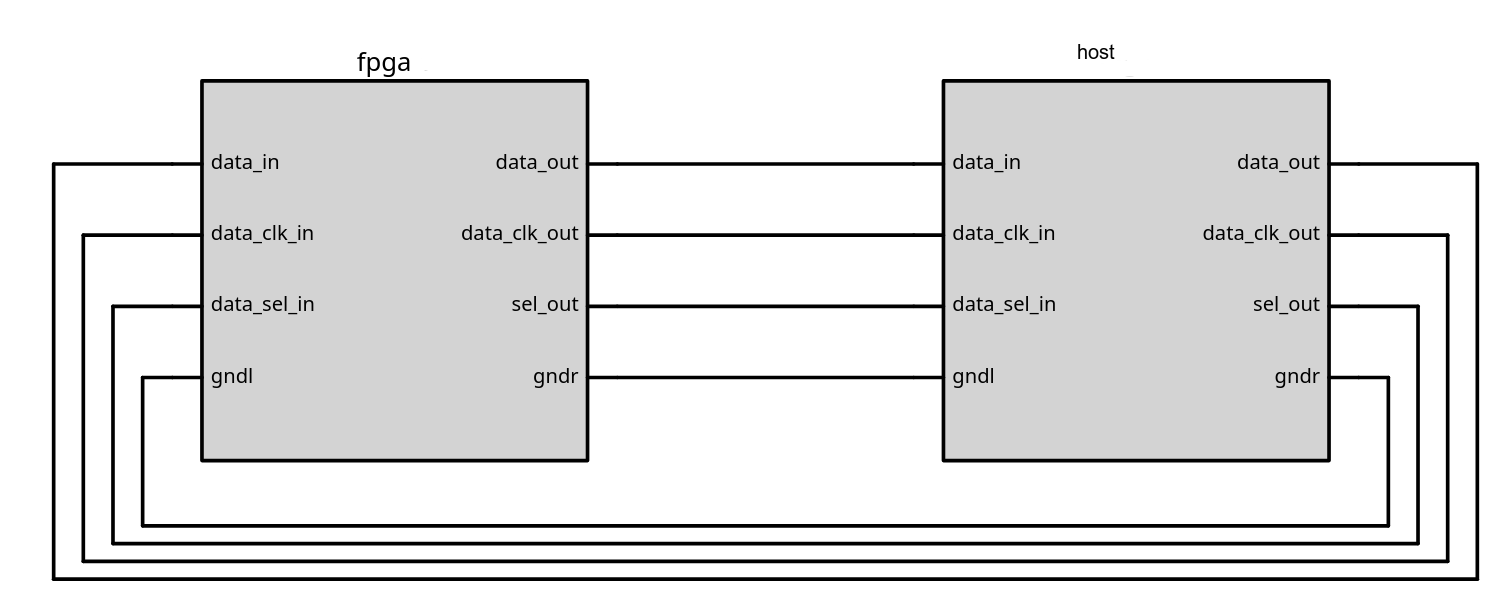
\includegraphics[width=14cm]{spi.png}

Source: lab 2, modified

The data out will connect directly to the priority queue dequeue port, cycling over the top n values. The receiver will be expected to decode the data and extract the n element cycle.

\section{Design Tradeoffs and Possible Issues}

There are some places where we have taken relatively naive approaches to modules. For instance, we are starting with a searchable FIFO for a priority queue, which is rather inefficient. After the minimal viable product is produced, we will consider other designs.  Another issue is that we have limited BRAM on our device. To process larger graphs, that can be from several Gb to Tb large, we would need to implement a DRAM buffer and SD Card usage. We would work on this after the minimal product deadline. For now, we will load graphs straight into BRAM, and if we were to run into size issues, we can make use of the lab's SPI module to fetch data from another machine.

\section{Deliverables}

\subsection{Timeline}
\begin{enumerate}
    \item Create CPU implementations of iQAN and graph sampling algorithms (already in progress, finish week of Oct 25)
    % \item Implement random sampler and distance calculation
    \item Implement n-dim distance calculator (week of Oct 31)
    \item Implement graph BRAM storage/cache (week of Oct 31 - Nov 7)
    \item Implement priority queue (week of Nov 7-14)
    \item Implement finding neighbors (week of Nov 7-14)
    \item Implement DRAM (week of Nov 7-21)
    \item Implement graph fetcher (week of Nov 14-21) %and cache and graph updater 
    \item Convert remaining parts of CPU implementation of vector search to Verilog/SystemVerilog (week of Nov 21)
    \item Integration of all parts (week of Nov 28)
    \item  Program sample use cases for testing performance and create reference implementations on CPU to evaluate performance on FPGA compared to CPU (week of Nov 28)
    \item Create a modular, dynamic implementation of our system (i.e. improvements for performance and usability) (week of Dec 6)
    \item Finish report (week of Dec 13)
\end{enumerate}

% We have specified how we tentatively expect to split components 2 and 3. We expect to have a better idea on how to split the work, including components 4, 5 and 6, in the next week or two after creating a block diagram of the modules and starting to build the system. 


\subsection{Goals}
For our minimal viable product, our goal is to create an FPGA-based accelerator for a graph-based vector search. The accelerator should be able to work on simple graphs and be faster than a CPU implementation. After that, we want to extend the minimal viable product to make a modular, variable-sized accelerator that can read large graphs from DRAM and SD cards.

% We currently see our project requiring modules to perform the following:
% \begin{enumerate}
%     \item Graph fetcher %and cache
%     % \item Graph walker
%     \item Distance calculation for n-dimensional vectors
%     \item Graph updater
%     \item Graph vector search (iQAN) % and graph pattern mining
%     \item Random graph point sampler to determine starting point (not necessary for minimal viable product)
% \end{enumerate}

% We expect these modules to change as we work more on the design phase of our accelerator. However, these modules, at a high level, are needed to build our system and are generally described earlier in this paper.

\section{Relevant Papers}

[1] iQAN: Fast and Accurate Vector Search with Efficient Intra-Query Parallelism on Multi-Core Architectures, 2023. \href{https://johnpzh.github.io/assets/papers/PPoPP-2023\_iQAN\_Zhen.CameraReady.pdf}{https://johnpzh.github.io/assets/papers/PPoPP-2023\_iQAN\_Zhen.CameraReady.pdf } (Primary paper reference)

[2] Co-design Hardware and Algorithm for Vector Search, 2023. \href{https://arxiv.org/pdf/2306.11182.pdf} {https://arxiv.org/pdf/2306.11182.pdf }

[3] NextDoor: Accelerating Graph Sampling for Graph Machine Learning Using GPUs, 2021. 
\newline \href{https://github.com/chenxuhao/ReadingList/blob/master/sampling/NextDoor.pdf}{https://github.com/chenxuhao/ReadingList/blob/master/sampling/NextDoor.pdf }

All diagrams are made by the students unless otherwise noted.

\end{document}
